% Chapter 1

\chapter{Introduction} % Main chapter title

\label{Chapter1} % For referencing the chapter elsewhere, use \ref{Chapter1} 

%----------------------------------------------------------------------------------------

% Define some commands to keep the formatting separated from the content 
\newcommand{\keyword}[1]{\textbf{#1}}
\newcommand{\tabhead}[1]{\textbf{#1}}
\newcommand{\code}[1]{\texttt{#1}}
\newcommand{\file}[1]{\texttt{\bfseries#1}}
\newcommand{\option}[1]{\texttt{\itshape#1}}

%----------------------------------------------------------------------------------------
Wind gusts are brief increases in wind speed (lasting seconds) compared to the mean wind speed over intervals of one or several minutes. The gust factor is defined as the peak gust divided by the mean wind speed over a specified time period. The peak wind gust is often defined as the highest 3-second rolling-average wind speed measured over a 10-minute period, while the mean wind speed is the average of all measurements in the same interval. This thesis uses that definition. However, definitions vary: for example, the US uses a 1-minute interval, leading to approximately 14\% higher values \cite{why_wind_gusts}.

The Navier–Stokes equation (\ref{eqn:navierstokes}) shows that changes in wind, both in time and space, depend on the pressure gradient, the oscillating force of the Earth (the Coriolis force), and frictional forces \cite{uncertainties_in_numerical_weather_predictions}.
\begin{equation}
    \label{eqn:navierstokes}
    \frac{\delta \mathbf{V}}{\delta t} + \mathbf{V}\cdot\nabla\mathbf{V} = \underbrace{-\frac{1}{\rho}\nabla P}_{\text{pressure}} -\overbrace{ f\mathbf{k}\times\mathbf{V}}^{\text{Coriolis}} - g - \underbrace{\frac{\delta(u'\omega')}{\delta z} - \frac{\delta(v'\omega')}{\delta z}}_{\text{resistance}}
\end{equation}

Traditionally, numerical weather prediction (NWP) systems are used to forecast and analyze weather patterns \cite{medium_range_3d_weather_forecasting_NN}. These models describe the evolution of discretized atmospheric states using partial differential equations grounded in physics. Forecasts are typically produced every hour, or at coarser intervals for climate simulations. With increasing computational power and efficiency, the trend is to output data more frequently \cite{GNP_vidtal}. However, such outputs summarize conditions over each period and may not capture short-term fluctuations well, including variations in wind speed and gusts \cite{canNNBeatNWP}.

This thesis examines methods to predict the gust factor using various predictors and multiple data sources, including NWP outputs and observational data. Accurate gust predictions are crucial, as it is often the peak wind gust that will cause damaging incidents, such as structural failures, traffic accidents and downed power lines. Moreover, the prevalence of extreme wind events is expected to increase in the future \cite{nasa_extreme_weather}.

\section{Background}

\subsection{Numerical weather prediction}
The history of numerical weather prediction dates back to the 1920s, when Lewis Fry Richardson pioneered the field and attempted to produce forecasts. His results were flawed due to numerical noise. The ENIAC, built in 1945, was a general-purpose computer used—among other tasks—for weather prediction. These forecasts took 24 hours to compute and predicted 24 hours into the future. While a proof of concept, they were not operationally useful \cite{TheENIACForecastsARecreation}. 

With the advent of electronic computers in the 1950s, the first operational forecasts emerged. In September 1954, Carl-Gustaf Rossby and his Stockholm-based team produced the first real-time barotropic forecasts. The following year, the Joint Numerical Weather Prediction Unit (JNWPU), based in Princeton, New Jersey, released its first 36-hour forecasts at 400, 700, and 900 mb. Although these forecasts were inferior to subjective human analyses, they demonstrated feasibility and spurred further development in the field \cite{historyNWP}. Since then, NWP has made tremendous strides in parallel with increases in computational power and efficiency.

\subsection{AI in weather forecasts}
In the last decade, there has been another transformation in weather prediction driven by artificial intelligence (AI). Interest in AI has come in waves: progress is made, then interest diminishes, but over the past 15 years growth has been steady. Notable drivers of this wave include advances in computational power (notably parallel processing on graphics processing units, GPUs), the development of neural networks (NNs) for processing massive datasets, and the availability of large online datasets. One type of NN is the convolutional neural network (CNN), originally designed for image processing but applicable to any gridded data with spatial structure \cite{canNNBeatNWP}. Since 2018, significant work has applied AI to weather prediction.

There are two common approaches to AI-based forecasting: combining NWP outputs with NNs, or using NNs alone. In the former, NWP forecasts can be used as inputs to NN training or integrated in other ways; in the latter, NNs are trained directly on meteorological observations, bypassing NWP entirely.

In 2018, Düben and Bauer showed that an NN could outperform a simple persistence forecast and compete with very coarse-resolution atmospheric models of similar complexity for short lead times \cite{dueben2018}. Also in 2018, Scher developed a deep CNN to emulate a general circulation model (GCM)—a numerical model representing physical processes—by training on GCM output. This approach allowed stable emulation of model dynamics for much longer horizons \cite{scher2018}. These papers were proofs of concept rather than production-ready replacements for NWP, but they demonstrated that deep-learning–based models could, with further development, compete with standard models in the field.

\subsection{Large weather models}
In the last two years, there have been even more developments with the emergence of Large AI Weather forecast Models (LWMs). In 2024, Ling et al.\ \cite{SecondRevolution} proposed a standardized definition of LWMs in meteorology, outlining three criteria, referred to as the "Three Large Rules":

\begin{enumerate}[label=\textbf{\arabic*}.,rightmargin=1.5em]
  \item \textbf{Large parameter count:} Typically ranging from tens of millions to billions of parameters.
  \item \textbf{Multiple predictands:} Forecasting at various levels (e.g., pressure or height levels) to provide detailed atmospheric vertical structure and surface conditions.
  \item \textbf{Scalability and downstream applicability:} Demonstrated, for example, by predicting cyclones even when not explicitly trained on cyclone data (e.g., \href{https://www.youtube.com/watch?v=PD1v5PCJs_o&ab_channel=GregBronevetsky}{GraphCast}) to showcase model versatility \cite{SecondRevolution}.
\end{enumerate}

Before 2022, LWMs had been shown to compete with traditional NWP in specific cases and to generate forecasts much faster after training, No model had been shown to be able to completely replace traditional NWP systems. In early 2022, Pathak et al.\ \cite{FourCastNet} introduced FourCastNet, which employs an Adaptive Fourier Neural Operator model leveraging transformer architecture instead of convolution. FourCastNet matches the performance of standard forecasting techniques at short lead times for large-scale variables and outperforms them for smaller-scale features. It generates a one-week forecast in under two seconds—orders of magnitude faster than conventional physical methods \cite{FourCastNet}. In 2022, several ML-based models demonstrated faster-than-NWP predictions after one-time training, with performance rivaling or exceeding NWP in some cases.

In 2023, Remi Lam and the GraphCast team at Google released GraphCast, which outperformed the European Centre for Medium-Range Weather Forecasts’ (ECMWF) industry-standard High-Resolution Forecast (HRES). GraphCast uses a graph-based representation instead of a regular grid, operating on a global latitude–longitude grid at 0.25° resolution, which introduces nonuniform point spacing near the poles; the graph structure helps mitigate this bias \cite{GraphCast}.

\subsection{Conclusion}
Substantial progress has been made since 2018 and especially since 2022 \cite{SecondRevolution}. The evolution from proof-of-concept ML methods to models competitive with—or surpassing—standard NWP has been remarkably rapid. It is important to note that training data for these large models are drawn from traditional NWP outputs, underscoring how ML and physics-based approaches can complement each other. The coming years promise further exciting developments in machine learning based weather prediction.

\section{Methodology and related work}\label{sec:methodology}

In this study, data from three sources are used:

\begin{enumerate}[label=\textbf{\arabic*}.,rightmargin=1.5em]
  \item Three-hourly reanalysis data for Iceland (2004–2023)
  \item Dense (20 by 20~m) gridded elevation data for Iceland
  \item Hourly observations from Icelandic meteorological stations
\end{enumerate}

The aim of the study is to improve prediction of gust factors that can be applied at any given place in Iceland. Currently, gust factor predictions can be obtained directly from NWP output, but one may also create a simple regression model (involving, e.g., wind speed and location) to predict them. To accomplish this, an NN is used as a backend to the NWP. The network is trained with gust factors from observations as ground truth, and model quality is measured by comparing predictions with either the NWP or the regression values. Note that only data at the prediction time is used; the time-series aspect of the data is not utilized.

In 2004, Hálfdán Ágústsson and Haraldur Ólafsson \cite{mean_gust_HA_HO} investigated gust factor variability in complex landscapes. They used data from automatic weather stations measuring wind at 10~m above ground during 1999–2001. They examined how three parameters affected the gust factor: \(d_m\), \(D\), and \(H\)—the wind direction relative to a mountain, the distance to the mountain, and the height of the mountain above the station. Their main results showed that the gust factor is inversely correlated with distance and directly correlated with mountain height. Ágústsson and Ólafsson considered the effect of a dominant point upwind but did not consider the broader landscape.

\subsection{Neural networks}
To capture patterns in the data, a neural network was constructed. An NN architecture was chosen because NNs handle complex data well and can manage large numbers of parameters. This flexibility is useful when training on different types of data and allows testing various network designs. An NN uses many matrix calculations to weight input parameters and predict an output. A deep neural network (DNN) has an input layer, an output layer, and one or more hidden layers. Hidden layers transform data from the input layer until it reaches the output layer. The input layer width equals the number of input parameters, and the output layer width equals the number of predictands.

\subsubsection{Structure of neural networks}
The general structure of a neural network is shown in Figure \ref{fig:nn_structure}. The input layer consists of $n$ neurons, each representing an input parameter. The output layer has $m$ neurons, each representing a predictand. Between these layers are one or more hidden layers, each with $h_i$ neurons, where $i$ is the layer index. Each neuron in a layer is connected to every neuron in the previous and next layers. The connections between neurons have weights that are adjusted during training to minimize prediction error.

\begin{figure}[H]
    \centering
    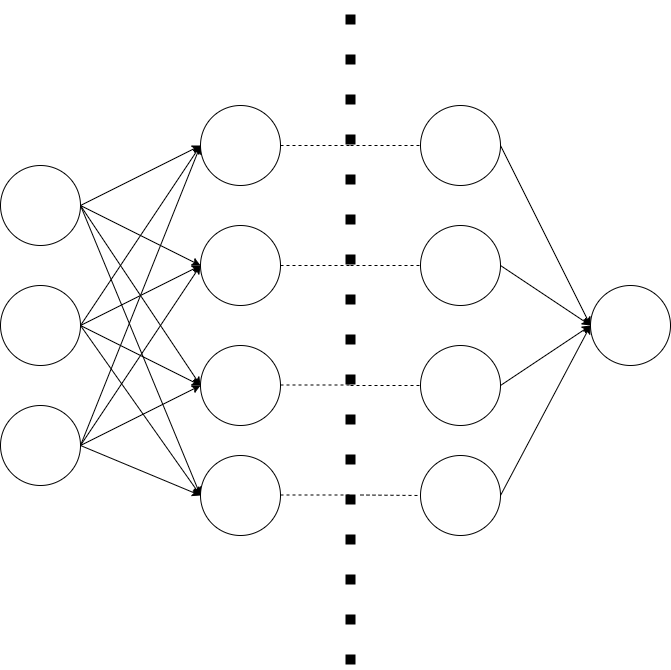
\includegraphics[width=0.8\textwidth]{figures/neural_network.drawio.png}
    \caption[General structure of a fully connected neural network]{General structure of a fully connected neural network. The figure shows a network with three input variables and one output variable. It also shows one hidden layer (and others are implied). This hidden layer has four neurons that each connect to all input neurons and all connect to all neurons in the next hidden layer (not shown). This continues for all hidden layers until the output layer, when there is only one neuron.}
    \label{fig:nn_structure}
\end{figure}

Models were created with different parameter sets to gauge each parameter’s influence. Each model produces a single numerical output. Every layer also has an activation function; common choices include Rectified Linear Unit (ReLU), Exponential Linear Unit (ELU), and hyperbolic tangent (tanh), defined in Equations (\ref{eqn:relu}), (\ref{eqn:elu}), and (\ref{eqn:tanh}).

\begin{equation}
    \label{eqn:relu}
    r(x):=\max(0, x)
\end{equation}

\begin{align}
    \label{eqn:elu}
    f(x) := x,\ x > 0\\
    f(x) := \alpha (e^x-1),\ x\leq 0,\ \alpha > 0
\end{align}

\begin{equation}
    \label{eqn:tanh}
    \operatorname{tanh}(x):=\frac{e^x-e^{-x}}{e^x+e^{-x}}
\end{equation}

These activation functions control neural activation and can help stabilize the network.
\subsection{Model evaluation}
To measure the performance of these models, both in training and testing, mean absolute percentage error (MAPE) as defined in Equation (\ref{eqn:mape}) was used.
\begin{equation}
    \label{eqn:mape}
    \text{MAPE} = \frac{1}{n}\sum_{i=1}^n\frac{|y_{\mathrm{predict}} - y_{\mathrm{true}}|}{y_{\mathrm{predict}}}
\end{equation}
This measure was chosen because the target is the gust factor (the wind gust over the average wind). If the target had been the wind gust rather than the gust factor, mean absolute error might be more appropriate.

\subsection{Model explainability}
Neural networks are often considered mysterious black boxes \cite{nn_black_box}. To understand model predictions, explainability methods are used. One such method is Shapley values \cite{shapley_information}. Shapley values are calculated as the average marginal contribution of a feature value across all possible coalitions. The contribution for a single feature \(j\) to a prediction \(\hat{f}(X)\) is given by Equation (\ref{eqn:shapley}). In Equation (\ref{eqn:shapley}), \(x_j\) is the feature value, \(\beta_j\) its weight, and \(\beta_j E[X_j]\) the mean effect estimate for feature \(j\).
\begin{equation}
    \label{eqn:shapley}
    \phi_j(\hat{f}) = \beta_j x_j - \beta_j E[X_j]
\end{equation}
For any combination of parameters, Shapley values explain the individual prediction by attributing a contribution to each feature. Other methods, like ELI5 (Explain Like I’m 5), randomly shuffle a feature and measure the effect on model performance \cite{eli5_information}.

Apart from aiding in understanding final constructed models and the role of individual features, such explainability measures can also be used to select features to use in the modelling. For example, if the computed Shapley distribution of a feature is clustered at 0, then the corresponding feature has little or no influence, and can be safely removed from the model.